\documentclass[11pt]{article}
\usepackage[letterpaper]{geometry}
\usepackage{MATH562}

\begin{document}
\noindent \textbf{\Large{Caleb Logemann \\
MATH 562 Numerical Analysis II \\
Final Exam
}}

%\lstinputlisting[language=Matlab]{H01_23.m}
\begin{enumerate}
    \item % #1 Done
        Let $A \in \RR^{m \times m}$ be written in the form $A = L + D + U$,
        where $L$ is strictly lower triangular, $D$ is the diagonal of $A$, and $U$
        is the strictly upper triangular part of $A$.
        Assuming $D$ is invertible, $A\v{x} = \v{b}$ is equivalent to
        $\v{x} = -D^{-1}\p{L + U}\v{x} + D^{-1}\v{b}$.
        The Jacobi iteration method for solving $A\v{x} = \v{b}$ is defined by
        \[
            \v{x}^{(n+1)} = -D^{-1}\p{L + U}\v{x}^{(n)} + D^{-1}\v{b}
        \]
        Show that if $A$ is nonsingular and strictly row diagonally dominant:
        \[
            0 < \sum{j \neq i}{}{\abs{a_{ij}}} < \abs{a_{ii}}
        \]
        then the Jacobi iteration converges to $\v{x}_* = A^{-1}\v{b}$ for each
        fixed $\v{b} \in \RR^m$.
        % Hint: the infinity norm is a convenient one to use

        \begin{proof}
            Let $\v{e}_n$ be the error of the nth iteration of the Jacobi iteration
            from the actual solution, that is let
            \[
                \v{e}_n = \v{x}^{(n)} - \v{x}_*.
            \]
            The Jacobi iteration converges to the real solution if
            \[
                \lim{n \to \infty}{\norm[\infty]{\v{e}_n}} = 0 
            \]
            The error vector can be expressed recursively by noting that
            $\v{x}^{(n)}$ is the Jacobi iteration evaluated on $\v{x}^{(n-1)}$
            and that $\v{x}_*$ is a fixed point of the Jacobi iteration as it is
            the true solution to the linear system.
            This means that
            \begin{align*}
                \v{x}^{(n)} &= -D^{-1}\p{L + U}\v{x}^{(n-1)} + D^{-1}\v{b} \\ 
                \v{x}_* &= -D^{-1}\p{L + U}\v{x}_* + D^{-1}\v{b}.
            \end{align*}
            Therefore we can express the error recursively as
            \begin{align*}
                \v{e}_n &= \v{x}^{(n)} - \v{x}_* \\
                \v{e}_n &= \p{-D^{-1}\p{L + U}\v{x}^{(n-1)} + D^{-1}\v{b}} - \p{-D^{-1}\p{L + U}\v{x}_* + D^{-1}\v{b}} \\
                \v{e}_n &= -D^{-1}\p{L + U}\v{x}^{(n-1)} + D^{-1}\p{L + U}\v{x}_* \\
                \v{e}_n &= -D^{-1}\p{L + U}\p{\v{x}^{(n-1)} - \v{x}_*} \\
                \v{e}_n &= -D^{-1}\p{L + U} \v{e}_{n-1}.
                \intertext{Extrapolating this backwards we see that $\v{e}_n$
                    can be expressed in terms of $\v{e}_0$}
                \v{e}_n &= \p{-D^{-1}\p{L + U}}^n \v{e}_{0}.
            \end{align*}
            Now we can consider the limit of $\norm[\infty]{\v{e}_n}$ as $n$
            goes to infinity.
            \begin{align*}
                \lim{n \to \infty}{\norm[\infty]{\v{e}_n}} &= \lim{n \to \infty}{\norm[\infty]{\p{-D^{-1}\p{L + U}}^n \v{e}_{0}}} \\
                \lim{n \to \infty}{\norm[\infty]{\v{e}_n}} &\le \norm[\infty]{\v{e}_{0}} \lim{n \to \infty}{\norm[\infty]{D^{-1}\p{L + U}}^n}
            \end{align*}
            Now consider $\norm[\infty]{D^{-1}\p{L + U}}$.
            The infinity norm is the max row sum of the matrix, that is
            \[
                \norm[\infty]{D^{-1}\p{L + U}} = \max*_{1 \le i \le m} \sum{j=1}{m}{\abs{\p{D^{-1}\p{L + U}}_{ij}}}
            \]
            Because $L + U = A - D$, $\p{L + U}_{ij} = a_{ij}$ if $i \neq j$ and $\p{L + U}_{ii} = 0$.
            Also $D^{-1}$ is diagonal with $\p{D^{-1}}_{ii} = \frac{1}{D_{ii}} = \frac{1}{a_{ii}}$.
            Therefore the matrix product $D^{-1}\p{L + U}$ has entries $\p{D^{-1}\p{L + U}}_{ij} = \frac{a_{ij}}{a_{ii}}$ if $i \neq j$ or 
            if $i = j$, then $\p{D^{-1}\p{L + U}}_{ii} = 0$.
            We can now say that
            \begin{align*}
                \norm[\infty]{D^{-1}\p{L + U}} &= \max*_{1 \le i \le m} \sum{j \neq k}{}{\abs{\frac{a_{ij}}{a_{ii}}}} \\
                \norm[\infty]{D^{-1}\p{L + U}} &= \max*_{1 \le i \le m} \frac{1}{\abs{a_{ii}}} \sum{j \neq k}{}{\abs{a_{ij}}}
                \intertext{However since $A$ is strictly row diagonally dominant $\abs{a_{ii}} > \sum{j \neq k}{}{\abs{a_{ij}}}$,
                    we can conclude that $\frac{1}{\abs{a_{ii}}} \sum{j \neq k}{}{\abs{a_{ij}}} < 1$. Therefore}
                \norm[\infty]{D^{-1}\p{L + U}} &< 1
            \end{align*}
            Since $\norm[\infty]{D^{-1}\p{L + U}} < 1$, it is true that
            $\lim{n \to \infty}{\norm[\infty]{D^{-1}\p{L + U}}^n} = 0$.
            Thus
            \begin{align*}
                \lim{n \to \infty}{\norm[\infty]{\v{e}_n}} &\le \norm[\infty]{\v{e}_{0}} \lim{n \to \infty}{\norm[\infty]{D^{-1}\p{L + U}}^n} \\
                \lim{n \to \infty}{\norm[\infty]{\v{e}_n}} &\le 0
            \end{align*}
            This shows that the error converges to zero, and this proves that
            the Jacobi iteration does converge to the true solution if $A$ is
            strictly row diagonally dominant.
        \end{proof}

    \item % #2 Done
        Let $A \in \RR^{m \times m}$ be symmetric positive definite (SPD),
        $\v{b} \in \RR^m$ and define $\phi:\RR^m \to \RR$ by
        \[
            \phi(\v{x}) = \frac{1}{2}\v{x}^T A \v{x} - \v{x}^T \v{b}
        \]
        Suppose $K$ is a subspace of $\RR^m$.
        Show that $\hat{\v{x}} \in K$ minimizes $\phi(\v{x})$ over $K$ if and
        only if $\nabla \phi(\hat{\v{x}}) \perp K$.

        \begin{proof}
            First let me describe $\nabla \phi(\v{x})$.
            \begin{align*}
                \nabla \phi(\v{x}) &=
                \begin{bmatrix}
                    \frac{\partial \phi}{\partial x_1} \\
                    \cdots \\
                    \frac{\partial \phi}{\partial x_m}
                \end{bmatrix} \\
                \frac{\partial \phi}{\partial x_i} &= \frac{\partial}{\partial x_i} \p{\frac{1}{2} \v{x}^T A \v{x} - \v{x}^T \v{b}} \\
                &= \frac{\partial}{\partial x_i} \p{\frac{1}{2} \sum{j = 1}{m}{x_j \sum{k = 1}{m}{a_{jk} x_k}} - \sum{j = 1}{m}{x_{j} b_j}} \\
                &= \frac{1}{2} \frac{\partial}{\partial x_i} \sum{j = 1}{m}{x_j \sum{k = 1}{m}{a_{jk} x_k}} - b_i \\
                &= \frac{1}{2} \frac{\partial}{\partial x_i} \p{x_i \sum{k = 1}{m}{a_{ik} x_k} + \sum{j \neq i}{}{x_j \sum{k = 1}{m}{a_{jk} x_k}}} - b_i \\
                &= \frac{1}{2} \p{\sum{k \neq i}{}{a_{ik} x_k} + 2a_{ii}x_i + \sum{j \neq i}{}{a_{ji} x_j}} - b_i \\
                &= \frac{1}{2} \p{\sum{k = 1}{m}{a_{ik} x_k} + \sum{j =  1}{m}{a_{ji} x_j}} - b_i \\
                &= \frac{1}{2} \p{\p{A\v{x}}_i + \p{A^T\v{x}}_i} - b_i
                \intertext{This is one entry of the vector $\nabla \phi(\v{x})$ therefore we can write the entire vector as}
                \nabla \phi(\v{x}) &= \frac{1}{2} \p{A\v{x} + A^T \v{x}} - \v{b}
                \intertext{Since $A$ is symmetric, $A = A^T$, this symplifies to}
                \nabla \phi(\v{x}) &= A\v{x} - \v{b}
            \end{align*}

            Now assume that $\nabla \phi(\hat{\v{x}}) \perp K$, therefore
            $\v{x} \cdot \p{A\hat{\v{x}} - \v{b}} = 0$ for any $\v{x} \in K$.
            Let $\v{x} \in K$, then $\v{x} = \hat{\v{x}} + \v{y}$ for some
            $\v{y} \in K$.
            \begin{align*}
                \phi(\v{x}) &= \phi(\hat{\v{x}} + \v{y}) \\
                &= \frac{1}{2}\p{\hat{\v{x}} + \v{y}}^T A \p{\hat{\v{x}} + \v{y}} - \p{\hat{\v{x}} + \v{y}}^T\v{b} \\
                &= \frac{1}{2}\p{\hat{\v{x}}^T + \v{y}^T} A \p{\hat{\v{x}} + \v{y}} - \hat{\v{x}}^T\v{b} - \v{y}^T\v{b} \\
                &= \frac{1}{2}\p{\hat{\v{x}}^TA + \v{y}^TA}\p{\hat{\v{x}} + \v{y}} - \hat{\v{x}}^T\v{b} - \v{y}^T\v{b} \\
                &= \frac{1}{2}\p{\hat{\v{x}}^TA\hat{\v{x}} + \hat{\v{x}}^TA\v{y} + \v{y}^TA\hat{\v{x}} + \v{y}^TA\v{y}} - \hat{\v{x}}^T\v{b} - \v{y}^T\v{b}
                \intertext{Note that $\hat{\v{x}}^TA\v{y} = \v{y}^TA^T\hat{\v{x}} = \v{y}^TA\hat{\v{x}}$ because $A$ is symmetric}
                &= \frac{1}{2}\p{\hat{\v{x}}^TA\hat{\v{x}} + 2\v{y}^TA\hat{\v{x}} + \v{y}^TA\v{y}} - \hat{\v{x}}^T\v{b} - \v{y}^T\v{b} \\
                &= \frac{1}{2}\hat{\v{x}}^TA\hat{\v{x}} - \hat{\v{x}}^T\v{b} + \v{y}^TA\hat{\v{x}} - \v{y}^T\v{b} + \frac{1}{2}\v{y}^TA\v{y} \\
                &= \frac{1}{2}\hat{\v{x}}^TA\hat{\v{x}} - \hat{\v{x}}^T\v{b} + \v{y}^T\p{A\hat{\v{x}} - \v{b}} + \frac{1}{2}\v{y}^TA\v{y} 
                \intertext{We know that $\nabla \phi(\hat{\v{x}}) \perp K$, therefore $\v{y}^T\p{A\hat{\v{x}} - \v{b}} = 0$}
                &= \frac{1}{2}\hat{\v{x}}^TA\hat{\v{x}} - \hat{\v{x}}^T\v{b} + \frac{1}{2}\v{y}^TA\v{y} \\
                &= \phi(\hat{\v{x}}) + \frac{1}{2}\v{y}^TA\v{y}
                \intertext{Since $A$ is positive definite $\v{y}^TA\v{y} \ge 0$ and therefore}
                \phi(\v{x}) \ge \phi(\hat{\v{x}})
            \end{align*}
            This $\hat{\v{x}}$ minimizes $\phi(\v{x})$ over $K$.

            Now assume that $\hat{\v{x}}$ minimizes $\phi(\v{x})$ over $K$, that
            is for any $\v{x} \in K$, $\phi(\hat{\v{x}}) \le \phi(\v{x})$.

            Let $\v{y} \in K$, then let $F(t) = \phi(\hat{\v{x}} + t \v{y})$.
            Note that $F(0) = \phi(\hat{\v{x}})$.
            Since $\hat{\v{x}}$ minimizes $\phi$ over $K$, $F(0) \le F(t)$ for
            any $t$.
            Thus $0$ is a minimizer of $F$ and $F'(0) = 0$.
            Using vector calculus
            \[
                F'(t) = \v{y}^T \nabla \phi(\hat{\v{x}} + t\v{y})
            \]
            Now using $t = 0$ we see that
            \begin{align*}
                F'(0) &= 0 \\
                \v{y}^T \nabla \phi(\hat{\v{x}}) &= 0
            \end{align*}
            Thus $\nabla \phi(\hat{\v{x}}) \perp K$, because $\v{y}^T \nabla \phi(\hat{\v{x}}) = 0$
            for any vector $\v{y} \in K$.
        \end{proof}

    \item % #3 Done
        Show that:
        \begin{enumerate}
            \item[(a)] % Done
                (Forward error analysis)
                \[
                    \abs{fl(\v{x}^T \v{a}) - \v{x}^T \v{a}} \le n \epsilon_{machine} \abs{\v{x}}^T \abs{\v{a}} + O(\epsilon_{machine}^2)
                \]
                where $\v{x}$ and $\v{a}$ are n-dimensional floating point vectors and
                $fl(\v{x}^T \v{a})$ represents the floating point computation of the dot
                product.

                \begin{proof}
                    I will prove by induction.
                    First consider the case when $n = 1$, then
                    \begin{align*}
                        \abs{fl(x a) - x a} &= \abs{x a (1 + \epsilon) - xa}
                        \intertext{Where $\epsilon = \epsilon_{machine} + O(\epsilon_{machine}^2)$}
                        &= \epsilon \abs{x} \abs{a} \\
                        &= 1 \epsilon_{machine} \abs{x} \abs{a} + O(\epsilon_{machine}^2)
                    \end{align*}
                    Assume that
                    \[
                        \abs{fl(\v{x}^T \v{a}) - \v{x}^T \v{a}} \le n \epsilon_{machine} \abs{\v{x}}^T \abs{\v{a}} + O(\epsilon_{machine}^2)
                    \]
                    for $n = 1, 2, \ldots, k$.
                    Now consider the case when $n = k+1$.
                    In this case $\v{x} = \br{\v{x}_k, x_{k+1}}^T$ and
                    $\v{a} = \br{\v{a}_k, a_{k+1}}^T$.
                    \begin{align*}
                        \abs{fl(\v{x}^T \v{a}) - \v{x}^T \v{a}} &= \abs{fl(\v{x}_k^T \v{a}_k + v_{k+1} a_{k+1}) - \v{x}_k^T \v{a}_k - v_{k+1} a_{k+1}} \\
                        &= \abs{\p{fl(\v{x}_k^T \v{a}_k) + fl(v_{k+1} a_{k+1})}(1 + \epsilon) - \v{x}_k^T \v{a}_k - v_{k+1} a_{k+1}} \\
                        &= \abs{fl(\v{x}_k^T \v{a}_k)(1 + \epsilon) - \v{x}_k^T \v{a}_k + fl(v_{k+1} a_{k+1})(1 + \epsilon) - v_{k+1} a_{k+1}} \\
                        &\le \abs{fl(\v{x}_k^T \v{a}_k)(1 + \epsilon) - \v{x}_k^T \v{a}_k} + \abs{fl(v_{k+1} a_{k+1})(1 + \epsilon) - v_{k+1} a_{k+1}} \\
                        &\le k \epsilon_{machine} \abs{\v{x}_k}^T \abs{\v{a}_k} + O(\epsilon_{machine}^2) + \abs{fl(v_{k+1} a_{k+1})(1 + \epsilon) - v_{k+1} a_{k+1}} \\
                        &\le k \epsilon_{machine} \abs{\v{x}_k}^T \abs{\v{a}_k} + O(\epsilon_{machine}^2) + (\epsilon_{machine})\abs{v_{k+1}} \abs{a_{k+1}} + O(\epsilon_{machine}^2) \\
                        &\le (k+1) \epsilon_{machine} \abs{\v{x}}^T \abs{\v{a}} + O(\epsilon_{machine}^2)\\
                    \end{align*}
                    Thus 
                    \[
                        \abs{fl(\v{x}^T \v{a}) - \v{x}^T \v{a}} \le n \epsilon_{machine} \abs{\v{x}}^T \abs{\v{a}} + O(\epsilon_{machine}^2)
                    \]
                    for all $n$.
                \end{proof}

            \item[(b)]
                Show that
                \[
                    \norm[F]{fl(XA) - XA} \le n \epsilon_{machine} \norm[F]{X} \norm[F]{A} + O(\epsilon^2_{machine})
                \]

                \begin{proof}
                    Each of the entries of $fl(XA)$ will be of the form $fl(\v{x}^T \v{a})$.
                    Therefore 
                    \[
                        \norm[F]{fl(XA) - XA} = \sqrt{\sum{i = 1}{n^2}{\p{fl(\v{x}^T \v{a}) - \v{x}^T\v{a}}^2}}
                    \]
                    From part (a)
                    \begin{align*}
                        \norm[F]{fl(XA) - XA} &\le \sqrt{\sum{i = 1}{n^2}{n^2 \epsilon^2_{machine} \p{\abs{\v{x}}^T \abs{\v{a}}}^2 + O(\epsilon_{machine}^4)}} \\
                        &\le n \epsilon_{machine} \sqrt{\sum{i = 1}{n^2}{x^2}} \sqrt{\sum{i = 1}{n^2}{a^2}} + O(\epsilon_{machine}^2) \\
                        &\le n \epsilon_{machine} \norm[F]{X} \norm[F]{A} + O(\epsilon_{machine}^2) \\
                    \end{align*}
                \end{proof}

            \item[(c)]
                Show that the relative backward error
                $\frac{\norm[F]{\delta A}}{\norm[F]{A}} \le n \kappa(A)O(\epsilon_{machine})$

                \begin{align*}
                    \frac{\norm[F]{\delta A}}{\norm[F]{A}} = \frac{\norm[F]{fl(XA) - XA}}{\norm[F]{A}} \\
                    = \frac{\norm[F]{X(A + \delta A) - XA}}{\norm[F]{A}} \\
                    &\le n \epsilon_{machine} \norm[F]{X} \norm[F]{A} \frac{1}{\norm[F]{A}} \\
                    &\le n \epsilon_{machine} \norm[F]{X} \\
                    &\le n \epsilon_{machine} \kappa(X) \\
                \end{align*}
        \end{enumerate}

    \item % #4 Done
        Let $A \in \RR^{n \times n}$ be a symmetric positive definite matrix.
        Let Gaussian elimination be carried out on $A$ without pivoting.
        After $k$ steps, $A$ will be reduced to the form
        \[
            A^{(k)} =
            \begin{pmatrix}
                A_{11}^{(k)} & A_{12}^{(k)} \\
                0            & A_{22}^{(k)} \\
            \end{pmatrix}
        \]
        where $A_{22}^{(k)}$ is an $(n - k) \times (n - k)$ matrix.
        Show by induction
        \begin{enumerate}
            \item[(a)]
                $A_{22}^{(k)}$ is symmetric positive definite.

                \begin{proof}
                    First I will prove by induction that $A_{22}^{(k)}$ is symmetric.
                    Consider the base case when $k = 0$, in this case
                    $A_{22}^{(0)} = A^{(0)} = A$, and since $A$ is symmetric $A_{22}^{(0)}$
                    is symmetric.
                    Now assume that $A_{22}^{(k)}$ is symmetric for
                    $k = 1, 2, \ldots, m-1$ with $m < n$.
                    Consider $A_{22}^{(m)}$.
                    We have from the Gaussian Elimination algorithm that
                    \begin{align*}
                        L^{(m)}A^{(m-1)} &= A^{(m)} \\
                        \begin{bmatrix}
                            1 &        &            &        &        &   \\
                              & \ddots &            &        &        &   \\
                              &        & 1          &        &        &   \\
                              &        & l_{m+1, m} & \ddots &        &   \\
                              &        & \vdots     &        & \ddots &   \\
                              &        & l_{n,m}    &        &        & 1
                        \end{bmatrix}
                        \begin{bmatrix}
                            A_{11}^{(m-1)} & A_{12}^{(m-1)} \\
                            0              & A_{22}^{(m-1)}
                        \end{bmatrix}
                        &=
                        \begin{bmatrix}
                            A_{11}^{(m)} & A_{12}^{(m)} \\
                            0            & A_{22}^{(m)}
                        \end{bmatrix}
                        \intertext{Looking at just the portion changing over this step.
                            I will relabel the matrices as follows.}
                        L &= 
                        \begin{bmatrix}
                               1           &        &        &   \\
                               l_{2, 1}    & \ddots &        &   \\
                               \vdots      &        & \ddots &   \\
                               l_{n-m-1,1} &        &        & 1
                        \end{bmatrix} \\
                        B &= A_{22}^{(m-1)} = \br{b_{ij}} \\
                        C &= A_{22}^{(m)} = \br{c_{ij}}
                        \intertext{Then the following matrix equation holds}
                        LB &= 
                        \begin{bmatrix}
                            b_{11} & \v{b}_{1,2:n-m-1}^T \\
                            \v{0}  & C
                        \end{bmatrix}
                    \end{align*}
                    Note that according to the Gaussian elimination algorithm
                    $l_{i1} = -b_{i1}/b_{11}$.
                    In order to show that $C$ which is $A_{22}^{(m)}$ is symmetric
                    we must show that $c_{ij} = c_{ji}$ for all $i$ and $j$.
                    We know that $c_{ij}$ is the $(i+1)$ row of $L$ dotted into
                    the $j+1$ column of $B$.
                    \begin{align*}
                        c_{ij} &= -l_{i+1,1} b_{1,j+1} + l_{i+1,i+1} b_{i+1,j+1} \\
                               &= -\frac{b_{i+1,1}}{b_{11}} b_{1,j+1} + 1 b_{i+1,j+1}
                        \intertext{From our inductive hypothesis $B$ is symmetric so $b_{i,j} = b_{j,i}$}
                               &= -\frac{b_{1,i+1}}{b_{11}} b_{j+1,1} + 1 b_{j+1,i+1} \\
                               &= -\frac{b_{j+1,1}}{b_{11}} b_{1,i+1} + l_{j+1,j+1} b_{j+1,i+1} \\
                               &= c_{ji}
                    \end{align*}
                    Therefore $c_{ij} = c_{ji}$ for all $i$ and $j$ and
                    $C = A_{22}^{(m)}$ is symmetric.
                    Thus by mathematical induction $A_{22}^{(k)}$ is symmetric
                    for all $k$.

                    Next I will prove that $A_{22}^{(k)}$ is positive definite.
                    Assume to the contradiction that $A_{22}^{(k)}$ is not
                    positive definite.
                    This implies that there exists a vector $\v{x}$ such that
                    $\v{x}^T A_{22}^{(k)} \v{x} \le 0$.
                    Construct $\v{y}$ such that $\v{y} \in \RR^m$ and the last
                    entries are $\v{x}$ and the first entries are $0$.
                    In this case because Gaussian elimination doesn't affect the
                    determinant
                    \begin{align*}
                        \v{y}^T A \v{y} &= \v{y}^T
                        \begin{bmatrix}
                            A_{11}^{(k)} & A_{12}^{(k)} \\
                            0            & A_{22}^{(k)}
                        \end{bmatrix}
                        \v{y} \\
                        &= \v{x}^T A_{22}^{(k)} \v{x} \\
                        &\le 0
                    \end{align*}
                    This contradicts the fact that $A$ is positive definite, therefore
                    $A_{22}^{(k)}$ must be positive definite for all $k$.
                \end{proof}

            \item[(b)] % Done
                $a_{ii}^{(k)} \le a_{ii}^{(k-1)}$ for all $k \le i \le n$,
                $k = 1, \cdots, n - 1$.

                \begin{proof}
                    In order to show this we must first find a formula for
                    $a_{ii}^{(k)}$.
                    By the Gaussian elimination algorithm without pivoting
                    \[
                        a_{ii}^{(k)} = a_{ii}^{(k-1)} - \frac{a_{i1}^{(k-1)}}{a_{11}^{(k-1)}} a_{1i}^{(k-1)}
                    \]
                    For a symmetric positive definite matrix
                    $a_{i1}^{(k-1)} = a_{1i}^{(k-1)}$, so this can be rewritten as
                    \[
                        a_{ii}^{(k)} = a_{ii}^{(k-1)} - \frac{\p{a_{i1}^{(k-1)}}^2}{a_{11}^{(k-1)}}
                    \]
                    It is known that $a_{11}^{(k-1)}$ is an eigenvalue of $A$ and since $A$ is positive definite
                    $a_{11}^{(k-1)} > 0$.
                    Also $\p{a_{i1}^{(k-1)}}^2 > 0$, therefore $\frac{\p{a_{i1}^{(k-1)}}^2}{a_{11}^{(k-1)}} > 0$.
                    This implies that $a_{ii}^{(k)} \le a_{ii}^{(k-1)}$, as subtracting a positive number makes
                    a number lower.
                \end{proof}
        \end{enumerate}

    \item % #5 Done
        Let $A \in \RR^{m \times n}$ with $m > n$ and
        \[
            A = 
            \begin{pmatrix}
                A_1 \\
                A_2
            \end{pmatrix}
        \]
        where $A_1$ is a nonsingular $n \times n$ matrix, and $A_2$ is an
        $(m - n) \times n$ arbitrary matrix.
        \begin{enumerate}
            \item[(a)] % Done
                What is the pseudo-inverse $A^+$ of $A$ such that $A^+ A = I_n$?
                Express it explicitly in terms of $A_1$ and $A_2$.

                The pseudo-inverse of $A$ is defined as
                \[
                    A^+ = (A^T A)^{-1} A^T
                \]
                Writing this in terms of $A_1$ and $A_2$ results in
                \begin{align*}
                    A^+ &=
                    \p{\begin{pmatrix}
                        A_1^T & A_2^T
                    \end{pmatrix}
                    \begin{pmatrix}
                        A_1 \\
                        A_2
                    \end{pmatrix}}^{-1}
                    \begin{pmatrix}
                        A_1^T & A_2^T
                    \end{pmatrix} \\
                    &= \p{A_1^T A_1 + A_2^T A_2}^{-1}
                    \begin{pmatrix}
                        A_1^T & A_2^T
                    \end{pmatrix}
                \end{align*}

            \item[(b)] % Done
                Prove that $\norm[2]{A^+} \le \norm[2]{A_1^{-1}}$.

                \begin{proof}
                    \begin{align*}
                        \norm[2]{A^{+}} &= \sup_{\v{b}} \frac{\norm[2]{A^+\v{b}}}{\norm[2]{\v{b}}}
                        \intertext{Let $P$ be the orthogonal projector onto the
                            range of $A$, then because $P$ is unitary and the
                            2-norm is unitarily invariant, $\norm[2]{\v{b}} = \norm[2]{P\v{b}}$.
                            Therefore}
                        \norm[2]{A^{+}} &= \sup_{\v{b}} \frac{\norm[2]{A^+\v{b}}}{\norm[2]{P\v{b}}}.
                        \intertext{Now considering the least squares problem
                            $\min*_{\v{x}}\norm[2]{A\v{x} - b}$, we know
                            that $A^+\v{b} = \v{x}$ and $P\v{b} = A\v{x}$.
                            Therefore}
                        \norm[2]{A^+} &= \sup_{\v{x}} \frac{\norm[2]{\v{x}}}{\norm[2]{A\v{x}}}.
                        \intertext{Note that}
                        A\v{x} &=
                        \begin{pmatrix}
                            A_1 \v{x} \\
                            A_2 \v{x}
                        \end{pmatrix} \\
                        \intertext{Therefore $\norm[2]{A\v{x}} \ge \norm[2]{A_1 \v{x}}$, so}
                        \norm[2]{A^{+}} &\le \sup_{\v{x}} \frac{\norm[2]{\v{x}}}{\norm[2]{A_1\v{x}}}.
                        \intertext{If we let $\v{y} = A_1\v{x}$, then $\v{x} = A_1^{-1}\v{y}$ and}
                        \norm[2]{A^{+}} &\le \sup_{\v{y}} \frac{\norm[2]{A_1^{-1}\v{y}}}{\norm[2]{\v{y}}} \\
                        &= \norm[2]{A_1^{-1}}
                    \end{align*}
                    Thus $\norm[2]{A^+} \le \norm[2]{A_1^{-1}}$.
                \end{proof}
        \end{enumerate}

    \item % #6 Done
        Let $A \in \CC^{m \times m}$ with $\rank(A) = r$.
        Suppose an SVD of $A$ is given by $A = U\Sigma V^*$, where
        $\v{u}_1, \v{u}_2, \ldots, \v{u}_m$ denote the columns of $U$ and
        $\v{v}_1, \v{v}_2, \ldots, \v{v}_m$ denote the columns of $V$.
        Prove that $\langle\v{v}_{r+1}, \ldots, \v{v}_m\rangle = \null(A)$.

        \begin{proof}
            First let $\v{x} \in \langle\v{v}_{r+1}, \ldots, \v{v}_m\rangle$, then
            $\v{x} = \sum{i = r+1}{m}{b_i \v{v}_i}$.
            If we let $b_i = 0$ for $i = 1, 2, \ldots, r$ and $\v{b} = \br{b_i}$,
            then $\v{x} = V\v{b}$.
            Now consider $A\v{x}$.
            \begin{align*}
                A\v{x} &= U\Sigma V^* V \v{b} \\
                       &= U \Sigma \v{b}
            \end{align*}
            However $\Sigma$ is a diagonal matrix with $\sigma_i$ along the
            diagonal, so $\p{\Sigma \v{b}}_i = \sigma_i b_i$.
            Since $A$ has $\rank(A) = r$, we know that $\sigma_i = 0$ for
            $i \ge r + 1$.
            Therefore if $1 \le i \le r$, then $\sigma_i b_i = 0$ because
            $b_i = 0$.
            If $r + 1 \le i \le m$, then $\sigma_i b_i = 0$ because
            $\sigma_i = 0$.
            Therefore we can conclude that $\Sigma \v{b} = \v{0}$
            Thus $A\v{x} = \v{0}$ and $\v{x} \in \null(A)$.

            Now assume that $\v{x} \in \null(A)$, that is $A\v{x} = \v{0}$.
            \begin{align*}
                A\v{x} &= \v{0} \\
                U\Sigma V* \v{x} &= \v{0} \\
                U^*U\Sigma V* \v{x} &= U^*\v{0} \\
                \Sigma V* \v{x} &= \v{0} \\
                \begin{bmatrix}
                    \sigma_1 \v{v}_1^* \v{x} \\
                    \cdots \\
                    \sigma_r \v{v}_r^* \v{x} \\
                    \sigma_{r+1} \v{v}_{r+1}^* \v{x} \\
                    \cdots \\
                    \sigma_m \v{v}_m^* \v{x}
                \end{bmatrix}
                &= \v{0}
                \intertext{Since $\sigma_i = 0$ for $r + 1 \le i \le m$}
                \begin{bmatrix}
                    \sigma_1 \v{v}_1^* \v{x} \\
                    \cdots \\
                    \sigma_r \v{v}_r^* \v{x} \\
                    0
                    \cdots \\
                    0
                \end{bmatrix}
                &= \v{0}
            \end{align*}
            This implies that $\v{v}_i^* \v{x} = 0$ for $1 \le i \le r$ since
            $\sigma_i > 0$ for $1 \le i \le r$.
            This is equivalent to $\v{x} \perp \v{v}_i$ for $1 \le i \le r$.
            Hence $\v{x} \in \langle \v{v}_1, \cdots, \v{v}_r \rangle^{\perp}$.
            Since $V$ is unitary
            \[
                \langle \v{v}_1, \cdots, \v{v}_r \rangle^{\perp} = \langle\v{v}_{r+1}, \ldots, \v{v}_m\rangle
            \]
            Thus $\v{x} \in \langle\v{v}_{r+1}, \ldots, \v{v}_m\rangle$.
        \end{proof}

    \item % #7 Done
        Problem 33.2 (Page 255) 
        Suppose algorithm 33.1 is executed for a particular $A$ and $\v{b}$
        until at some step $n$, an entry $h_{n+1, n} = 0$ is encountered.
        \begin{enumerate}
            \item[(a)]
                Show how (33.13) can be simplified in this case.
                What does this imply about the structure of a full $m \times m$
                Hessenberg reduction $A = QHQ^*$ of $A$?

                This implies that $H$ is
                \[
                    H =
                    \begin{bmatrix}
                        H_n & X
                    \end{bmatrix}
                \]
                where $X$ can be anything and $Q$ is $Q_n$ extended to an
                orthonormal basis.

            \item[(b)] % Done
                Show that $K_n$ is an invariant subspace of $A$, i.e., $AK_n \subseteq K_n$.

                \begin{proof}
                    Let $\v{x} \in AK_n$, then $\v{x} = A\v{y}$ where $\v{y} \in K_n$.
                    If $\v{y} \in K_n$, then $\v{y} = \sum{i = 1}{n}{y_i \v{q}_i}$.
                    This implies that
                    \[
                        \v{x} = \sum{i = 1}{n}{y_i A\v{q}_i}
                    \]
                    For $1 \le i \le n-1$, $A\v{q}_i \in K_n$.
                    Consider $A\v{q}_n$, equation 33.4 states
                    \begin{align*}
                        A\v{q}_n &= h_{1n} \v{q}_1 + \cdots + h_{nn} \v{q}_n + h_{n+1,n} \v{q}_{n+1}
                        \intertext{Since $h_{n+1,n} = 0$}
                        A\v{q}_n &= h_{1n} \v{q}_1 + \cdots + h_{nn} \v{q}_n
                    \end{align*}
                    Thus $A\v{q}_n \in K_n$ as well.
                    This implies that $x = A\v{y} \in K_n$.
                    Thus $AK_n \subseteq K_n$.
                \end{proof}

            \item[(c)] % Done
                Show that if the Krylov subspaces of $A$ generated by $\v{b}$
                are defined by $K_k = \langle \v{b}, A\v{b}, \ldots, A^{k-1}\v{b} \rangle$,
                then $K_n = K_{n+1} = K_{n+2}$.

                \begin{proof}
                    In part (b) we showed that $AK_n \subseteq K_n$.
                    Obviously $K_{n+1} = AK_n$, so $K_{n+1} \subseteq K_n$.
                    Clearly from the definition $K_n \subseteq K_{n+1}$ as
                    any vector in $\langle \v{b}, A\v{b}, \ldots, A^{n-1}\v{b} \rangle$ will
                    also be in $\langle \v{b}, A\v{b}, \ldots, A^{n}\v{b} \rangle$.
                    Thus $K_n = K_{n+1}$.
                    This can also be applied for any $m > n$, $K_m = A^{m-n}K_n$, and
                    therefore $K_m \subseteq K_n$.
                    So clearly $K_n = K_m$ for any $m > n$.
                \end{proof}

            \item[(d)] % Done
                Show that each eigenvalue of $H_n$ is an eigenvalue of $A$.

                Let $\lambda$ be an eigenvalue of $H_n$, then there exists
                a nonzero eigenvector $\v{x}$ such that $H_n \v{x} = \lambda \v{x}$.
                From equation 33.12 we know that $H_n = Q^*_n A Q_n$.
                This implies that
                \begin{align*}
                    Q^*_n A Q_n \v{x} &= \lambda \v{x} \\
                    A Q_n \v{x} &= \lambda Q_n \v{x}
                    \intertext{Let $\v{y} = Q_n \v{x}$}
                    A \v{y} &= \lambda \v{y}
                \end{align*}
                Thus $\lambda$ is also an eigenvalue of $A$.

            \item[(e)] % Done
                Show that if $A$ is nonsingular, then the solution $\v{x}$ to the system
                of equations $A\v{x} = \v{b}$ lies in $K_n$.

                Since the eigenvalues of $A$ are the same as the eigenvalues
                of $H_n$, if $A$ is nonsingular than $H_n$ is also nonsingular.
                Furthermore
                \begin{align*}
                    A^{-1} &= \p{Q_n H_n Q_n^*}^{-1} \\
                    A^{-1} &= Q_n H_n^{-1} Q_n^*\\
                \end{align*}
                Therefore
                \begin{align*}
                    \v{x} &= A^{-1}\v{b} \\
                          &= Q_n H_n^{-1} Q_n^* \v{b} \\
                          &= Q_n \p{H_n^{-1} Q_n^* \v{b}} \\
                \end{align*}
                This shows that $\v{x}$ is a linear combination of the
                columns of $Q_n$ which form a basis of $K_n$.
                Therefore $\v{x} \in K_n$.
        \end{enumerate}

    \item % #8 Done
        Problem 36.1 (Page 283)
        In Lecture 27 it was pointed out that the eigenvalues of a symmetric
        matrix $A \in \RR^{m \times m}$ are the stationary values of the
        Rayleigh quotient $r(\v{x}) = (\v{x}^TA\v{x})/(\v{x}^T \v{x})$ for
        $\v{x} \in \RR^m$.
        Show that the Ritz values at step $n$ of the Lanczos iteration are the
        stationary values of $r(\v{x})$ if $\v{x}$ is resticted to $K_n$.

        \begin{proof}
            The Ritz values are the eigenvalues of $T_n$ the tridiagonal matrix.
            In this case $A = Q_n^* T_n Q_n$.
            So if $\v{y} = Q_n \v{x}$ is an eigenvector of $T_n$, with a corresponding Ritz
            value, then
            \begin{align*}
                r(\v{x}) &= \frac{\v{x}^T A \v{x}}{\v{x}^T \v{x}} \\
                &= \frac{\v{x}^T Q_n^* T_n Q_n \v{x}}{\v{x}^T \v{x}} \\
                &= \frac{\v{x}^T Q_n^* T_n Q_n \v{x}}{\v{x}^T Q_n^* Q_n \v{x}} \\
                &= \frac{\v{y}^T T_n \v{y}^T}{\v{y}^T \v{y}} \\
            \end{align*}
            This is the Ritz value associated with $\v{y}$ at the nth step,
            so the Ritz values are stationary for the Rayleigh quotient.
        \end{proof}

    \item % #9 Done
        Let $f:\RR \to \RR$ be twice continuously differentiable for all $x$ in
        the neighborhood $\set{x \in \RR | \abs{x - \xi} < r}$ of a simple zero
        $\xi$ of $f$ such that $f(\xi) = 0$.
        Consider the two-step Newton method:
        \[
            y_k = x_k - f(x_k)/f'(x_k), \quad x_{k+1} = y_k - f(y_k)/f'(x_k).
        \]
        \begin{enumerate}
            \item[(a)] % Done
                Show that if the method converges, then
                \[
                    \lim{k \to \infty}{\frac{x_{k+1} - \xi}{(y_k - \xi)(x_k - \xi)}} = \frac{f''(\xi)}{f'(\xi)}
                \]

                \begin{proof}
                    First we assume that the method converges, this implies that
                    \begin{align*}
                        \lim{k \to \infty}{x_k - \xi} &= 0
                        \intertext{and}
                        \lim{k \to \infty}{y_k - \xi} &= 0
                    \end{align*}
                    Also the problem will use the Taylor expansion of $f(y_k)$ and
                    $f'(x_k)$ about $\xi$, so these will be stated here for later use.
                    \begin{align*}
                        f(y_k) &= f(\xi) + (y_k - \xi) f'(\xi) + O((y_k - \xi)^2) \\
                               &= (y_k - \xi) \p{f'(\xi) + O(y_k - \xi)} \\
                        f'(x_k) &= f'(\xi) + (x_k - \xi)f''(\xi) + O((x_k - \xi)^2)
                    \end{align*}
                    Now I will consider the limit
                    \begin{align*}
                        &\lim{k \to \infty}{\frac{1}{(y_k - \xi)(x_k - \xi)} \p{x_{k+1} - \xi}} \\
                        &= \lim{k \to \infty}{\frac{1}{(y_k - \xi)(x_k - \xi)} \p{y_k - \xi - \frac{f(y_k)}{f'(x_k)}}} \\
                        &= \lim{k \to \infty}{\frac{1}{(y_k - \xi)(x_k - \xi)} \p{y_k - \xi - \frac{(y_k - \xi) \p{f'(\xi) + O(y_k - \xi)}}{f'(x_k)}}} \\
                        &= \lim{k \to \infty}{\frac{1}{(x_k - \xi)} \p{1 - \frac{f'(\xi) + O(y_k - \xi)}{f'(x_k)}}} \\
                        &= \lim{k \to \infty}{\frac{1}{(x_k - \xi)} \p{1 - \frac{f'(\xi) + O(y_k - \xi)}{f'(\xi) + (x_k - \xi)f''(\xi) + O((x_k - \xi)^2)}}} \\
                        %&= \lim{k \to \infty}{\frac{1}{(x_k - \xi)} \p{\frac{f'(\xi) + (x_k - \xi)f''(\xi) + O((x_k - \xi)^2)}{f'(\xi) + (x_k - \xi)f''(\xi) + O((x_k - \xi)^2)} - \frac{\p{f'(\xi) + O(y_k - \xi)}}{f'(\xi) + (x_k - \xi)f''(\xi) + O((x_k - \xi)^2)}}} \\
                        &= \lim{k \to \infty}{\frac{1}{(x_k - \xi)} \p{\frac{f'(\xi) + (x_k - \xi)f''(\xi) + O((x_k - \xi)^2) - f'(\xi) - O(y_k - \xi)}{f'(\xi) + (x_k - \xi)f''(\xi) + O((x_k - \xi)^2)}}} \\
                        &= \lim{k \to \infty}{\frac{1}{(x_k - \xi)} \p{\frac{(x_k - \xi)f''(\xi) + O((x_k - \xi)^2) - O(y_k - \xi)}{f'(\xi) + (x_k - \xi)f''(\xi) + O((x_k - \xi)^2)}}} \\
                        &= \lim{k \to \infty}{\frac{f''(\xi) + O((x_k - \xi)) - O((y_k - \xi)/(x_k - \xi))}{f'(\xi) + (x_k - \xi)f''(\xi) + O((x_k - \xi)^2)}}
                        \intertext{Taking the limit results in}
                        &= \frac{f''(\xi)}{f'(\xi)}
                    \end{align*}
                \end{proof}

            \item[(b)] % Done
                The convergence is cubic:
                \[
                    \lim{k \to \infty}{\frac{x_{k+1} - \xi}{(x_k - \xi)^3}} = \frac{1}{2}\p{\frac{f''(\xi)}{f'(\xi)}}^2
                \]

                \begin{proof}
                    In this proof I will use the Taylor expansions of $f(x_k)$
                    and $f'(x_k)$ around $\xi$, so I will state them here
                    \begin{align*}
                        f(x_k) &= f(\xi) + (x_k - \xi) f'(\xi) + O((x_k - \xi)^2) \\
                               &= (x_k - \xi) \p{f'(\xi) + O(x_k - \xi)} \\
                        f'(x_k) &= f'(\xi) + (x_k - \xi)f''(\xi) + O((x_k - \xi)^2)
                    \end{align*}
                    Now consider the limit
                    \begin{align*}
                        \lim{k \to \infty}{\frac{x_{k+1} - \xi}{(x_k - \xi)^3}}
                        &= \lim{k \to \infty}{\frac{x_{k+1} - \xi}{(y_k - \xi)(x_k - \xi)} \frac{y_k - \xi}{(x_k - \xi)^2}}
                        \intertext{From part (a)}
                        &= \frac{f''(\xi)}{f'(\xi)} \lim{k \to \infty}{\frac{y_k - \xi}{(x_k - \xi)^2}}
                    \end{align*}
                    Now consider this limit individually
                    \begin{align*}
                        &\lim{k \to \infty}{\frac{y_k - \xi}{(x_k - \xi)^2}} \\
                        &= \lim{k \to \infty}{\frac{1}{(x_k - \xi)^2}\p{x_k - \xi - \frac{f(x_k)}{f'(x_k)}}} \\
                        &= \lim{k \to \infty}{\frac{1}{(x_k - \xi)^2}\p{x_k - \xi - \frac{(x_k - \xi) \p{f'(\xi) + \frac{1}{2}(x_k - \xi) f''(\xi) + O\p{(x_k - \xi)^2}}}{f'(x_k)}}} \\
                        &= \lim{k \to \infty}{\frac{1}{x_k - \xi}\p{1 - \frac{f'(\xi) + \frac{1}{2}(x_k - \xi) f''(\xi) + O\p{(x_k - \xi)^2}}{f'(x_k)}}} \\
                        &= \lim{k \to \infty}{\frac{1}{x_k - \xi}\p{1 - \frac{f'(\xi) + \frac{1}{2}(x_k - \xi) f''(\xi) + O\p{(x_k - \xi)^2}}{f'(\xi) + (x_k - \xi)f''(\xi) + O((x_k - \xi)^2)}}}
                        \intertext{By finding a common denominator and adding the fractions}
                        &= \lim{k \to \infty}{\frac{1}{x_k - \xi}\p{\frac{\frac{1}{2}(x_k - \xi) f''(\xi) + O\p{(x_k - \xi)^2}}{f'(\xi) + (x_k - \xi)f''(\xi) + O((x_k - \xi)^2)}}} \\
                        &= \lim{k \to \infty}{\frac{\frac{1}{2}f''(\xi) + O\p{x_k - \xi}}{f'(\xi) + (x_k - \xi)f''(\xi) + O((x_k - \xi)^2)}} \\
                        \intertext{Taking the limit}
                        &= \frac{1}{2} \frac{f''(\xi)}{f'(\xi)}
                    \end{align*}
                    Now going back to the original limit
                    \begin{align*}
                        \lim{k \to \infty}{\frac{x_{k+1} - \xi}{(x_k - \xi)^3}} &= \frac{f''(\xi)}{f'(\xi)} \lim{k \to \infty}{\frac{y_k - \xi}{(x_k - \xi)^2}} \\
                        \lim{k \to \infty}{\frac{x_{k+1} - \xi}{(x_k - \xi)^3}} &= \frac{1}{2} \p{\frac{f''(\xi)}{f'(\xi)}}^2 \\
                    \end{align*}
                \end{proof}
        \end{enumerate}

    \item % #10 Done
        MATLAB project

        Below are the function for performing the 
        Jacobi method, the Gauss-Seidel Method, and the Conjugate Gradient
        method.
        \lstinputlisting[language=Matlab]{Jacobi.m}
        \lstinputlisting[language=Matlab]{GaussSeidel.m}
        \lstinputlisting[language=Matlab]{ConjugateGradient.m}

        The following script uses these three methods to solve the diffusion
        equation $-u_{xx} = 1$ on $x \in \p{0, 1}$.
        It also plots the residual against the number of iterations.
        \lstinputlisting[language=Matlab]{H05.m}
        \begin{center}
            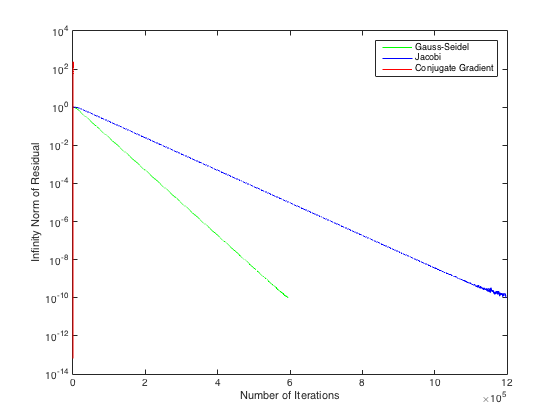
\includegraphics[scale=.7]{Figures/05_10_1.png}
        \end{center}

        We see in this plot that the Gauss-Seidel method converges much faster
        than the Jacobi method.
        Both of these experience linear convergence, but Gauss-Seidel is a faster
        linear convergence.
        The Conjugate Gradient method converges much faster than either of the
        stationary methods.
        The Conjugate Gradient method converges in only 250 steps which is less
        than $m = 500$, the size of the matrix.
\end{enumerate}
\end{document}
